
\begin{figure*}[t]
\centering
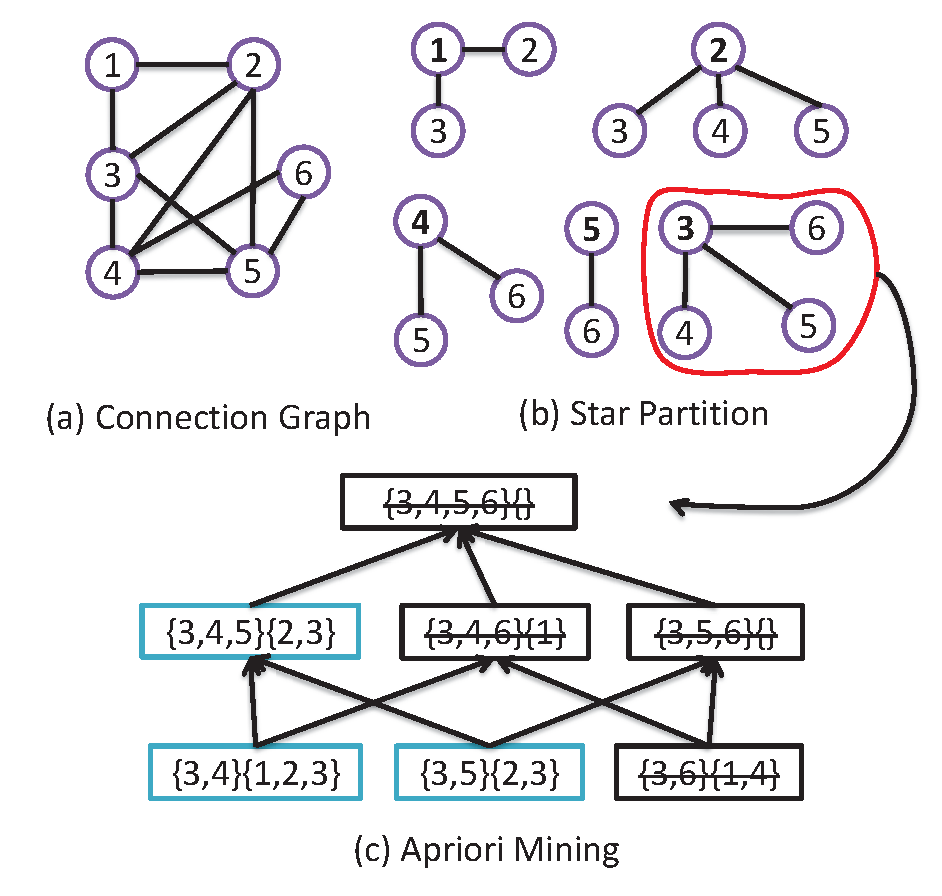
\includegraphics[width=0.9\textwidth]{spm.eps}
\caption{Star partition and mining. (a) Conceptual connection graph from Figure 1.(b) Five star partitions are generated
(c) Apriori Mining with various pruning techniques.}
\label{fig:star_partition}
\end{figure*}

\section{SPARE: Star Partitioning and Apriori Enumerator}
\label{sec:spm}
The aforementioned replicate partitioning is based on the temporal dimension 
and results in groups of snapshots in each partition. 
To resolve the limitations caused by the replicate partitioning, 
we propose a new Star Partitioning and ApRiori Enumerator, named SPARE, 
to replace the second cycle of map-reduce jobs in Figure~\ref{fig:trm}. 
Our new parallel mining framework is shown in Figure~\ref{fig:star_partition}. 
Its input is the set of clusters generated in each snapshot and the output 
are mined GCMP patterns. In the following, we explain the two major components: 
star partitioning and apriori enumerator.


\subsection{Star Partitioning}
Let $G_t$ be a graph for snapshot $S_t$, in which each node 
is a moving object and two objects are connected if they appear 
in the same cluster. It is obvious that $G_t$ consists of a set of small cliques. 
Based on $G_t$, we define an aggregated graph $G_A$ to summarize the 
cluster relationship among all the snapshots. In $G_A$, two objects
form an edge if they are connected in any $G_t$s. Furthermore, 
we attach an inverted list for each edge, 
storing the associated timestamps in which the two objects are connected. 
An example of $G_A$, built on the trajectory database in Figure~\ref{fig:related_work}, 
is shown in Figure~\ref{fig:star_partition} (a). 
As long as two objects are clustered in any timestamp, they are connected in $G_A$. 
The object pair $(o_1,o_2)$ appears in two clusters at timestamps 
$2$ and $3$ and is thus associated with an inverted list $\{2,3\}$.


We use \emph{star} as the data structure to capture the pair relationships. 
To avoid duplication, as $G_t$ is an undirected graph and an edge may appear in multiple stars, 
we enforce a global ordering among the objects and propose a concept named \textit{directed star}.

\begin{definition}[Directed Star]
Given a vertex with global id $s$, its directed star $Sr_s$ is defined as the set of neighboring vertices with global id $t>s$. $s$ is also called star id.
\end{definition}

Given an aggregated graph $G_A$, we can enumerate all the possible stars, 
as shown in  Figure~\ref{fig:star_partition} (b). These stars are emitted 
from mappers to different reducers. The key is the star ID and the value 
is the neighbors in the star as well as the associated inverted lists. 
The reducer will then call the Apriori-based algorithm to enumerate all the valid GCMP patterns.


Before we introduce the Apriori enumerator, we are interested to 
examine the issue of global ordering on the moving objects.
This is because assigning different IDs to the objects will result in 
different star partitioning results, which will eventually affect the workload 
balance among the map-reduce jobs. Specifically, we intended to 
measure the size of the \emph{stragglers}~\cite{kwon2012skewtune,xin2013shark,coppa2015data}
in star partition. Intuitively, the \emph{stragglers} are the partitions that
takes the most time to execute. We use $\Gamma$ to indicate the number of edges
of the \emph{straggler} in star partition. And smaller $\Gamma$ is always preferred.
%Specifically, if there are partitions
%taking significant long time to execute, they would become
%the bottleneck of the entire system. Such long time-taken partitions
%are referred as \emph{stragglers}~\cite{kwon2012skewtune,xin2013shark,coppa2015data}
%We use $\Gamma$ to indicate the number of edges
%of the largest \emph{straggler} in star partition. Intuitively,
%a large $\Gamma$ means the system has a more prominent bottleneck. 
%And smaller $\Gamma$ is always preferred.
For example, Figure~\ref{fig:star-alt} gives two star partitioning results under 
different vertex ordering on the same graph. The top one has the $\Gamma = 5$ while
the bottom one has the $\Gamma = 3$.
It is obvious that the bottom one is much more balanced in terms of the size of each partition.


%An important concern in design parallel algorithms is the distribution of work loads.  
%Traditionally, the quality of a partition strategy 
%is measured based on two aspects: (1) the number of result partition, which
%affects the maximum parallelism
%(2) the size balance of partitions, which affects the finishing
%time of a job. Unlike TRM where each partition
%contains equal-sized snapshots, the size distribution 
%of stars in SPM remains unknown.
%Nevertheless, we notice that, in SPM, the total sizes of 
%stars are invariant. Therefore, the quality of a star partition
%can be formalized as the \emph{skewness}, which is the maximum star size
%among all stars. Smaller \emph{skewness} naturally results in more partitions
%and less imbalance.
%}

\begin{figure}[h]
\centering
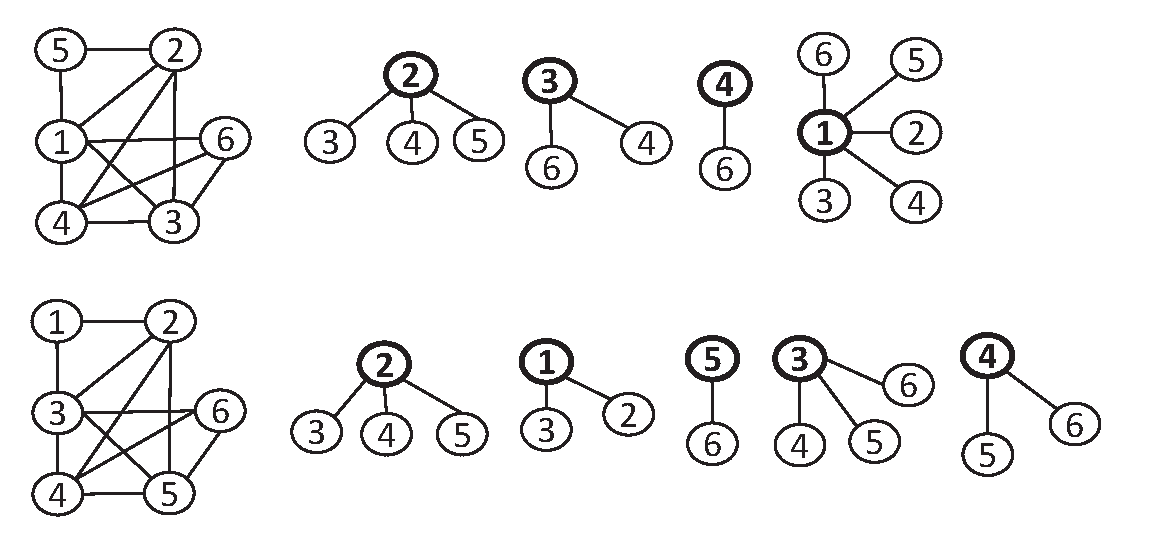
\includegraphics[width=0.5\textwidth]{star-alt.eps}
\caption{Examples of star partitioning with different vertex ordering.}
\label{fig:star-alt}
\end{figure}


To determine the optimal vertex orders with the objective of minimizing $\Gamma$, 
we can use a linear algebra model as follows:  
Let $G_A$ be an aggregate graph, with a $n \times n$ adjacent matrix $J$.
A vertex order is in fact a permutation of $J$. Therefore,
the adjacent matrices of any reordered graphs can be represented as $PJP^T$
where $P \in \mathbb{P}$ is a 
\emph{permutation matrix}~\footnote{an identity matrix with rows shuffled} with dimension $n$.
Since in star partition, we assign each edge $e(i,j)$ in $G_A$ to the lower vertex, 
then the matrix $B=\triu(PJP^T)$~\footnote{\text{triu} is the upper triangle part of a matrix}
represents the assignment matrix wrt. $P$ (i.e., $b_{i,j} = 1$ if vertex $j$ is in star $Sr_i$).
Let vector $\vec{b}$ be the \textit{one}\footnote{every element in $\vec{b}$ is $1$} 
vector of size $n$. Let $\vec{c} = B\vec{b}$, then each $c_i$ 
denotes the number of edges in star $Sr_i$. Thus, $\Gamma$ can be represented
as the infinity norm of $B\vec{b}$. Let $\Gamma^*$ be the minimum $\Gamma$ among all vertex orders. 
$\Gamma^*$ can then be formulated as follows:
\begin{equation}
\Gamma^* = \min_{P \in \mathbb{P}}{||B\vec{b}||_\infty} \text{ ,where } ||B\vec{b}||_\infty = \max_{1\leq j \leq n}(c_j)
\end{equation}

It is challenging to directly optimize the above equation. 
First, suppose there are $n!$ permutation matrices. 
Such a high complexity is trivially unpractical. Second,
since $G$ is unknown in prior,
the vertex order cannot be planned beforehand. 
Despite these challenges, we find a simple $O(1)$ time 
solution which is good enough as stated in the 
following theorem.

\begin{theorem}[Balance of Star Partition]
\label{THM:SPM_LB}
Let $G$ be an aggregated graph with $n$ vertexes and the average degree $d$.
Let $\Gamma^*$ be optimal size of straggler among all vertex orders.
Let $\Gamma$ be the size of straggler wrt an random vertex order $P$. 
With high probability, the difference between $\Gamma$ and $\Gamma^*$ is $O(\sqrt{n \log n})$.
That is,  with probability $1-1/n$, 
$\Gamma = \Gamma^* + O(\sqrt{n \log n})$.
\end{theorem}

In fact, we have a tighter bound of $(\Gamma - \Gamma^*)$ if 
the aggregate graph is \emph{dense}. Specifically, if $d\geq \sqrt{12\log n}$, with
high probability, $\Gamma = \Gamma^* + O(\sqrt{d\log n})$.
Utilizing Theorem~\label{THM:SPM_LB}, in star partition, it is safe 
to choose the object IDs as the vertex order. This because real object IDs are often 
hashed and can be deemed as random.


%
%Even though the TRM algorithm works in a parallel way, it requires to replicate the data $\eta$ times. 
%When $\eta$ is small, TRM perform good parallelism. However, wh
%
%When handling \emph{swarm}, \emph{group} and \emph{platoon} patterns, $\eta$ has to be set to $|\mathbb{T}|$ to guarantee correctness, resulting in very expensive data replication overhead. 
%%Handling those cases are equivalent to replicate the entire snapshots to each partition, 
%%which surrenders the benefit of parallelism.
\eat{
Although TRPM works in a parallel way, we observe two inefficiencies. First, the
performance of TRPM largely relies on $\eta$ which further depends on pattern parameters.
When $\eta$ is large, the shuffle and reduce cost of TRPM is high. Second, 
the parallel execution of line sweep algorithm may discover the same pattern from
multiple partitions, which introduces redundant work. To resolve the two limitations,
we design a novel \emph{Star Partition and Mining} algorithm.
}
%After computing the star, each partition is applied with a reduce task. 
%Indeed, a star $Sr_s$ can be viewed as a subset of original trajectories. 
%This is done by treating each vertex in $Sr_s$ as an object. 
%The time sequence of $s$ is the union of all edges in $Sr_s$. 
%And the time sequence of $v \neq s$ is the edge $(s,v)$. Therefore, we
%are able to mine stars from the similar trajectory concepts.

\subsection{Apriori Enumerator}
Intuitively, given a GCMP pattern with an object set $\{o_1,o_2,\ldots,o_m\}$, all the pairs of $(o_i,o_j)$ with $1\leq i<j\leq m$ must be connected in the associated temporal graphs $\{G_t\}$. This inspires us to leverage the classic Apriori algorithm to enumerate all the valid GCMP patterns starting from pairs of objects. However, we observe that the monotonicity property does not hold between an object set and its supersets.

\begin{example}
In this example, we show that if an object set is not a valid pattern, we cannot prune all its super sets.
Consider two candidates $P_1=\{o_1,o_2:1,2,3,6\}$ and $P_2=\{o_1,o_3:1,2,3,7\}$. 
Let $L=2,K=3,G=2$, then both candidates are not valid patterns. 
However, the timestamps of their super set $\{o_1,o_2,o_3\}$ is $P_1.T \cap P_2.T=\{1,2,3\}$, which
conform to $L,K,G$. This indicates that even though $P_1.O$ and $P_2.O$ are not valid patterns, they
cannot be pruned. Otherwise, $\{o_1,o_2,o_3\}$ would be missed out.
\end{example}   

\subsubsection{Monotonicity}
To ensure monotonicity, we first introduce a procedure named \textit{star simplification}, to reduce the number of edges as well as unnecessary timestamps in the inverted lists. For instance, if the size of the inverted list for an edge $e$ is smaller than $K$, then the edge can be safely removed because the number of timestamps in which its supersets are clustered must also be smaller than $K$. To generalize the idea, we propose two concepts named \textit{maximal $G$-connected subsequence} and \emph{candidate sequence}.

\begin{definition}[Maximal $G$-connected Subsequence]
A sequence $T'$ is said to be a maximal $G$-connected subsequence of $T$ if (1) $T'$ is the subsequence of $T$, i.e., $\exists i\leq j, T' = T(i,\ldots,j)$ , (2) $T'$ is $G$-connected, and (3) there exists no other subsequence $T''$ of $T$ such that $T'$ is the subsequence of $T''$ and $T''$ is G-connected.
\end{definition}
%Hence, our idea is to examine the validity of object pairs. If $(o_i,o_j)$ itself is not a valid GCMP pattern, then all the supersets containing $(o_i,o_j)$ can be pruned. For instance, $(XXX,XXX)$ are not connected in Figure~\ref{} and all its supersets can be pruned.

\begin{example}
Let $G=2$, consider $T_1=(1,2,4,5,6,9,10,11,13)$. $T$ has two maximal $2$-connected subsequences:
$T_1^A=\{1,2,4,5,6\}$ and $T_1^B=\{9,10,11,13\}$. Consider $T_2=(1,2,4,5,6,8,9)$,
it can be verified that it is $2$-connected, thus $T_2$ has only one maximal $2$-connected subsequence which is
itself.
%Let $G = 2$, sequence $T_1=(1,2,4,5,6,9,10,11,13)$ and $T_2=(1,2,4,5,6,8,9)$
%%
% XXX EXPLAIN HOW TO DERIVE THE MAXIMAL G-CONNECTED SUBSEQUENCES OF $T_1$ and $T_2$. 
\end{example}


\begin{definition}[Candidate Sequence]
$T$ is a candidate sequence if for any of its maximal $G$-connected subsequence $T'$, we have (1) $T'$ is $L$-consecutive; and (2) $|T'|\geq K$.
\end{definition}

\begin{example}
Let $L = 2, K = 4$ and we follow the above example. $T_1$ is not a candidate sequence
since one of its maximal $2$-connected subsequence (i.e., $T_1^B$) is not $2$-consecutive.
In contrast, $T_2$ is a candidate sequence because it has one maximal $2$-connected subsequence
and it is $L$-connected with size greater than $2$.
\end{example}

%Not that, although $T_1$ is not a candidate sequence, it can be simplified
%to a candidate sequence (i.e, $T_2$). Generally, for any time sequence $T$, 
%if it does not contain a \emph{candidate sequence}, then it cannot contribute
%to any valid patterns. In fact, only the candidate sequence inside $T$ affects
%the final patterns. Therefore, we may use the candidate sequence to simplify edges in 
%a star. During the simplification, if an edge results in a candidate
%sequence of size zero, then it is removed from the star. Otherwise,
%the simplified edge is kept. By so doing, the size of the new star
%is much smaller.

\begin{definition}[Sequence Simplification]
Given a sequence $T$ and the GCMP parameters $G,L,K$, a $T^\#$ is
the simplified sequence of $T$ if (1) $T^\#$ is contained in $T$, i.e., $T\# \subseteq T$.
(2) $T^\#$ is a candidate sequence, and (3) no other candidate sequence
$T^\#_1$ is contained in $T$ and contains $T^\#$.
%GIVEN A SEQUENCE, PLEASE UNIQUELY DEFINE ITS SIMPLIFICATION OUTPUT.
\end{definition}
Note that, not every $T$ has the simplified sequence.  For example, if $L =3$,
then the simplified sequence of $(1,2,5,6)$ does not exists.
Nevertheless, if there exists a $T^\#$ of $T$, then $T^\#$ is unique
as stated in the following theorem:
\begin{theorem}
For any sequence $T$, if $T$'s simplified sequence is not empty, then
there exists a unique $T^\#$ wrt $T$.
\end{theorem}

\begin{proof}
We prove by contradiction. Suppose there are two simplified sequences $T_A^\#$ and $T_B^\#$ of the same $T$. We prove that, unless $T_B^\# \equiv T_A^\#$, $T_A^\#$ can always be enlarged, which leads to a contradiction. For simplicity, we use $\overline{ab}$ to denote the segment of a sequence from timestamp $a$ to timestamp $b$.
Consider the timestamps $T_C=T_B^\# - T_A^\#$. If $T_C = \emptyset$, then $T_A^\# \equiv T_B^\#$ naturally. Next, consider an arbitrary consecutive segment $\overline{ef}$ in $T_C$. Without loss of generality, we assume the next $G$-connected segment of $\overline{ef}$ in $T_B^\#$ is $\overline{cd}$ and the previous $G$-connected segment is $\overline{gh}$. There are four cases to be considered. We demonstrate the cases in Figure~\ref{fig:proof_thm_3}:
\begin{figure}[h]
\centering
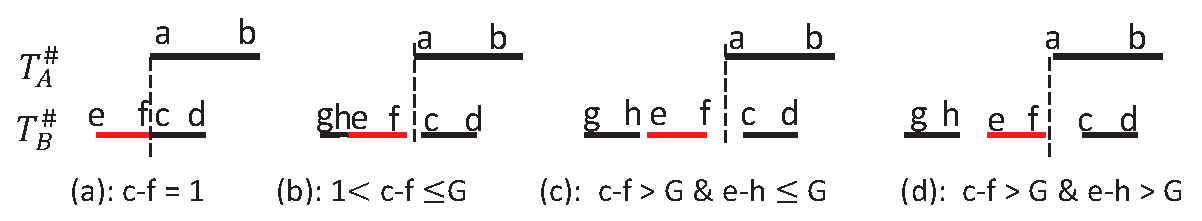
\includegraphics[width=0.45\textwidth]{thm3proof.eps}
\caption{Proof of theorem 3.}
\label{fig:proof_thm_3}
\end{figure}
\begin{itemize}
\item Case (a): $c-f = 1$, that is $\overline{ef}$ is part of a longer consecutive segment $\overline{ed}$. Since timestamp $c$ is in $T_A^\#$, $T_A^\#$ can be safely enlarged by adding $\overline{ef}$.
\item Case (b): $G \geq c-f> 1$. In this case, since $c\geq a$, then $a-f \leq G$. Since the size of $\overline{ef}$ is greater or equal to $L$, adding $\overline{ef}$ to $\overline{ab}$ would still result in a valid candidate sequence.
\item Case (c): $c-f > G$ and $e-h \leq G$. In this case, $\overline{ef}$ belongs to a $G$-connected sequence $\overline{gf}$ in $T_B^\#$. Observe that $\overline{gh}$ has no intersection with $T_A^\#$ (otherwise, it backs to case (a)), adding $\overline{gf}$ to $T_A^\#$ is equivalent in adding another candidate sequence to $T_A^\#$, making $T_A^\#$ still a valid simplified sequence.
\item Case (d): $c-f > G$ and $ e- h > G$. In this case, since $\overline{ef}$ is part of $T_B^\#$ and there is no segments $G$-connected with $\overline{ef}$, $\overline{ef}$ itself must be a candidate sequence. Therefore adding $\overline{ef}$ to $T_A^\#$ would still enlarge $T_A^\#$.
\end{itemize}
\end{proof}



Next, we design an efficient simplification process with linear complexity.
It takes two rounds scan of $T$ as shown in Algorithm~\ref{algo:simp_prune}. 
In the first round, the consecutive portions of $T$ with size less than $L$ are removed.
In the second round, the maximal $G$-connected sequences of size less than $K$ are removed. 

\begin{algorithm}
\caption{Edge Simplification}
\label{algo:simp_prune}
\begin{algorithmic}[1]
\Require $T$
\State{---$L$ Phase---}
\State $c \gets 0$
\For {$i \in (0,...,|T|)$}
	\If{$T[i] - T[i-1] > 1$} 
		\If{$i - c < L$} 
			\State $T$ remove $[c:i)$
		\EndIf
		\State $c \gets i$
	\EndIf
\EndFor
\State{---$G$-$K$ Phase---}
\State $s\gets 1$, $c\gets 0$
\For{$i \in (0: |T|)$}
	\If{$T[i] - T[i-1] > G$}
		\If{$s < K$}   
			\State $T$ remove $[c:i)$
		\EndIf
		\State {$c \gets i$, $s \gets 1$}
	\Else
		\State $s++$
	\EndIf
\EndFor
\end{algorithmic}
\end{algorithm}

\begin{example}
Take $T_1=\{1,2,4,5,6,9,10,11,13\}$ as an example of edge simplification. Let $L = 2, K = 4, G = 2$.
In the first round of scan. $T_1$ reduces to $\{1,2,4,5,6,9,10,11\}$. The consecutive subsequence $\{13\}$
is removed by $L=2$. $T_1$ has two maximal $2$-consecutive subsequences, which 
are $\{1,2,4,5,6\}$ and $\{9,10,11\}$. Since $K=4$, $\{9,10,11\}$ is removed
from $T_1$ in the second round of scan. Therefore, $T_1$ is simplified to $\{1,2,4,5,6\}$, which is shortened $44\%$.
\end{example}


With the concepts of \textit{candidate sequence} and \textit{sequence simplification}, we are ready to define the monotonic property that can be used for pruning.
\begin{theorem}\label{THM:SPM_TM}
Given a candidate pattern $P=\{O:T\}$, if sequence $P.T$ cannot be simplified to a candidate sequence, then any pattern candidate $P'$ with $P.O \subseteq P'.O$ can be pruned.
\end{theorem}

\begin{proof}
Let $P_2$ be a true pattern with $P_2.O \supseteq P.O$. It is easy to see that $P_2.T \subseteq P.T$. Since $P_2.T$ conforms to $G,L,K$. This indicates that $P_2.T$ is indeed a candidate sequence. Since $P_2.T \subseteq P.T$, $P.T$ can be simplified to candidate sequence (i.e., to $P_2.T$) which contradict with the fact that $P$ cannot be simplified. Thus no such true pattern exists.
\end{proof}

%IN THE PROOF, YOU NEED TO SHOW 1) $P$ IS NOT VALID 2) ALL THE SUPERSETS OF $P.O$ ARE NOT VALID.












\subsubsection{Apriori Algorithm}

To systematically discover valid patterns in each star, 
we design the \emph{Apriori Mining} algorithm. 
To describe the  algorithm, we call a candidate pattern $R$-pattern 
if the size of its object set is $R$.  Therefore, each edge
in the star is effectively a $2$-pattern. The intuition of Apriori mining
is the observation that $(R+1)$-patterns can be generated
from $R$-patterns and $2$ patterns. Thus, we may iteratively 
enumerate pattern candidates with all possible sizes.
In particular, initially, for each $e(s,v)=ET$, pattern $p=(\{s,v\}, ET)$ is formed. 
During each iteration, we generate $(R+1)$-patterns by joining $R$-patterns 
with the $2$-patterns. Technically, the join between $p_1=(O_1:T_1)$ and $p_2=(O_2:T_2)$
generates a new pattern $p_3=(O_1 \cup O_2:T_1 \cap T_2)$. Note that in $Sr_s$,
each $R$-pattern contains the object $s$, thus the join only 
grow a $R$-pattern at most to a $(R+1)$-pattern.
Our mining algorithm stops where no further patterns are generated. 
The algorithm is illustrated as in Algorithm~\ref{algo:apriori_mining}.

\begin{algorithm}
\caption{Apriori Mining}
\label{algo:apriori_mining}
\begin{algorithmic}[1]
\Require{$Sr_s$}
\State { Lv $\gets \{\}$,Ground $\gets \{\}$, Output $\gets \{\}$}
\ForAll{$e(s,t) = T \in Sr_s$}
\State{Simply $e(s,t)$} \Comment{ Simplification}
\State {Ground.add($\langle \{s,t\}, T \rangle$)}
\State {Lv $\gets$ Ground}
\EndFor
\While{Lv is not empty}
		\State {Lv $\gets$ Lv $\oplus $ Ground} \Comment{ Simplification}
		\State {Remove false patterns in Lv}
		\Comment{Monotonicity}
		\If{union of Lv is a valid pattern}
			\State{output.add(Lv)} \Comment{Forward Closure}
			\State{break}
		\EndIf
\EndWhile
\State output.addAll($Lv$)
\State \Return output
\end{algorithmic}
\end{algorithm}
 
An illustration of Algorithm~\ref{algo:apriori_mining} is shown in Figure~\ref{fig:star_partition} (c).
As shown, the star $Sr_3=\{3,4,5,6\}$ initially generate three $2$-candidates. At every iteration, 
higher level candidates are generated by joining lower level candidates. When no more candidates 
can be generated, the algorithm stops by outputting the valid patterns.
%
%It is notable that, in star partition, original data is 
%replicated at most $O(|\mathbb{O}|)$ times.
%In later sections, we will describe several 
%more optimization techniques to further reduce the amount of replicated data.




%In such a way, 
%given an object $u$, all the objects potentially
%co-moved with $u$ are captured in $u$'s neighborhood, which
%forms a \emph{star} structure in graph terms. SPM utilizes
%such structures to partition objects and then adapts an Apriori 
%algorithm to discover true GCMPs from each partition.






EXPLAIN CLEARLY HOW YOU IMPLEMENT THE FORWARD CLOSURE CHECKING! BETTER SHOW IT IN THE ABOVE PSEDUDO CODE IN THE APRIORI ALGORITHM.

Although leveraging \emph{temporal monotonicity} could largely prune
false candidates and reduce the apriori search space, 
it is ineffective when a \textit{true} pattern exists. 
In an extreme case, if a final pattern of a star $Sr_s$ is 
the \textit{union of all vertices} in the star,
then in apriori, ${|Sr_s|}\choose{i + 1}$ candidates needs to be generated at 
each level $i$. This results in an exponential search space while
the output only contains one pattern.  
Generally, when candidates at level $i$ collectively forms a true pattern, 
running aprior produces many wasted candidates. 

Let $Lv_i$ be the set of candidates at level $i$ of Algorithm~\ref{algo:apriori_mining},
we use the \emph{forward closure} $FC_i$ to denote the union of the objects in
all candidates in $Lv_i$. Then, the \emph{forward closure checking} is stated as follows:
\begin{theorem}[Forward Closure Checking]
\label{THM:SPM_FCC}
Let $Lv_i$ be the candidates generated at level $i$ in Algorithm~\ref{algo:apriori_mining},
if $FC_i$ is a proper pattern, then it is safe to terminate Algorithm~\ref{algo:apriori_mining}
and directly output $FC_i$.
\end{theorem}


It is notable that, as the level grows in Algorithm~\ref{algo:apriori_mining}, the closure $FC$
reduces, thus the terminating power of $FC$ would be stronger. We give hybrid example of the three
optimization as follows:
%To facilitate efficient mining, we adapt the \emph{forward closure checking} rule to 
%quickly determine whether it is sufficient to terminate the apriori search. Given the candidates at
%level $i$ $Lv_i$, we define the \emph{forward closure} of $Lv_i$ as the union of objects from
%all candidates. Then, the following \emph{forward closure checking} rule can be used:
%
%\begin{theorem}[Forward Closure Checking Rule]
%Let $Lv_i$ be the candidates generated at level $i$ in Algorithm~\ref{algo:apriori_mining}, the forward closure
%is $\mathbb{F}_i = \cup_{cand \in Lv_i} (cand.O) $. Algorithm~\ref{algo:apriori_mining} terminates when 
%$FC_i$ forms a valid GCMP .
%\end{theorem}

\begin{example}
We use Figure~\ref{fig:star_partition} (c) to 
demonstrate the power of candidate pruning. 
As shown, at the initial stage, $\{3,6:3\}$ is first pruned by \textit{Edge Simplification} since its
timestamps fails to be a candidate sequence. Subsequently, all further candidates containing $\{3,6\}$ 
are pruned by \textit{Temporal Monotonicity}. Then, we check the \textit{Forward Closure} 
of remaining candidates (i.e., $\{3,4\}$ and $\{3,5\}$) and find $\{3,4,5\}$ is a
valid candidate. Therefore, $\{3,4\}$ and $\{3,5\}$ are pruned, and $\{3,4,5\}$ is the output.
\end{example}






\subsection{Correctness of SPARE}
We summarize the workflow of SPARE framework in Figure~\ref{fig:star_partition} as follows. After the parallel clustering in each snapshot, we build an aggregated graph $G_A$ to capture the clustering relationship. In the map phrase, we partition $G_A$ into stars and emit the star partitions to the reducers. Each reducer is an Apriori Enumerator. When receiving a star $Sr_i$, the reducer creates initial candidate patterns. Specifically, for each $o \in Sr_i$, a pattern candidate $\{o,i: e(o,i)\}$ is created. Then the Apriori algorithm enumerate the true patterns from the candidate patterns. Meanwhile, the \emph{simplification}, \emph{monotonicity pruning} and \emph{forward closure checking} are applied to boost the enumeration process.
\eat{ ADD THE DETAILS WHEN THE REDUCER RECEIVE THE STAR PARTITIONS. HOW THEY DERIVE THE FINAL RESULT PATTERNS.}


\eat{
\begin{algorithm}
\caption{Star Partition and Mining}
\label{algo:spm_overview}
\begin{algorithmic}[1]
\Require list of $\langle t, S_t \rangle$ pairs
\State {---Map phase---}
\label{code:spm-map-start}
\ForAll{$C \in S_t$}
	\ForAll {$(o_1 ,o_2) \in C \times C$}
		\If{$o_1 < o_2$}  \label{code:spm-edge-direct}
			\State emit a $\langle o_1, o_2, \{t\}\rangle$ triplet
		\EndIf
	\EndFor
\EndFor
\label{code:spm-map-end}

\State {---Partition and Shuffle phase---}
\label{code:spm-shuffle-start}
\ForAll{$\langle o_1, o_2, \{t\}\rangle$ triplets} 
	\State group-by $o_1$, emit $\langle o_1, Sr_{o_1} \rangle$ 
	%\State group-by $o_2$, emit $\langle o_2, Sr_{o_2} \rangle$
\EndFor
\label{code:spm-shuffle-end}

\State {---Reduce phase---}
\label{code:spm-reduce-start}
\ForAll{$\langle o, Sr_{o} \rangle$}
\State Apriori($Sr_o$)
\EndFor
\label{code:spm-reduce-end}

\end{algorithmic}
\end{algorithm}
}


In the following, we show the correctness of the SPARE framework.
\begin{theorem}
\label{THM:SPM_CORRECT}
The SPARE framework guarantees completeness and soundness.
\end{theorem}
\begin{proof}
If $P$ is a valid pattern in original trajectories, 
let $s$ be the object with smallest ID in $P.O$. 
Based on the definition of GCMP, $\forall t \in P.T$, $\forall o \in P.O$, $C_t(s) = C_t(o)$.
It follows that all object $o \in P.O$ are in $Sr_s$. 
Furthermore, every timestamp in $P.T$ is included
in $Sr_s$. Therefore, $P$ is a valid pattern in $Sr_s$. This ensures the \emph{completeness}. For any pattern $P$ enumerated by SPARE, by definition of star partition, $\forall o_1, o_2 \in P.O$, $\forall t \in P.T$, $C_t(o_1) = C_t(o_2)$. This ensure the \emph{soundness}.
\end{proof}.

In fact, besides that every valid patterns can be
mined in some stars, star partition further ensures
that patterns discovered
from different star partitions cannot be the same. 
This can be formulated as:

\eat{It is also interesting to observe that no duplicate patterns will be generated from the star partitions.}
\begin{lemma}[Pattern Uniqueness of Star Partition]
\label{LEM:SPM_CORRECT}
Let $Sr_i$ and $Sr_j$ ($i\neq j$) be two star partitions. Let $P_i$ (resp. $P_j$) be 
the patterns discovered from $Sr_i$ (resp. $Sr_j$). 
Then, $\forall p_i \in P_i, \forall p_j \in P_j$, we have $p_i.O \not\equiv p_j.O$.
\end{lemma}
\begin{proof}
The correctness of Lemma~\ref{LEM:SPM_CORRECT} can be directly derived from the above arguments:
let $o_i$ be the smallest element in $p_i.O$ and $o_j$ be the smallest element in $p_j.O$. 
Since $p_i$ and $p_j$ belongs to different stars, then $o_i \neq o_j$, 
therefore $p_i.O \not\equiv p_j.O$. This proves the lemma.
\end{proof}

This lemma verifies the superiority of the SPARE framework over the TRPM framework.

